\subsection{Genauigkeit- und Updategeschwindigkeitsvergleich}
  
  \begin{figure}[h]
    \begin{center}
    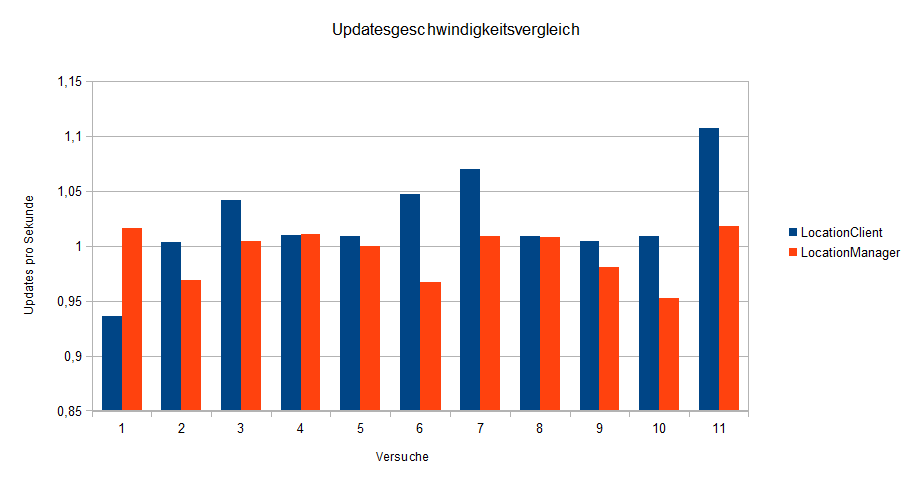
\includegraphics[width=1.0\textwidth]{4-Technische_Loesungen/4-1-Positionsermittlung/Data/updates_per_second_bigger.png}
    \end{center}
     \caption{Updates pro Sekunde}
     \label{fig: picUdates}
  \end{figure}
	
	\begin{figure}[h]
    \begin{center}
    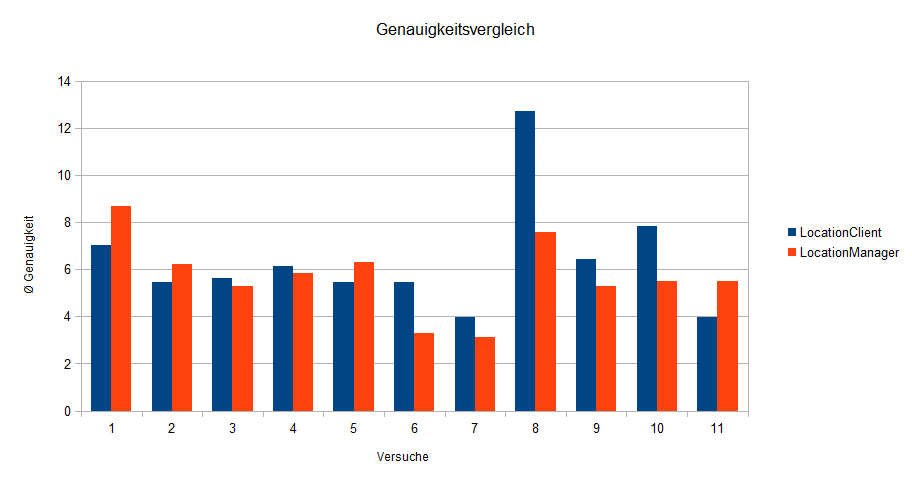
\includegraphics[width=1.0\textwidth]{4-Technische_Loesungen/4-1-Positionsermittlung/Data/accuracy_bigger.png}
    \end{center}
     \caption{Genauigkeit}
     \label{fig: picAccu}
  \end{figure}
	  
\clearpage

Die Auswertung der Daten hat ergeben, dass bzgl. der Genauigkeit der LocationManager in 6 von 11 Versuchen besser als der LocationClient abschneitet. Im Bezug auf Updates pro Sekunde liefert der LocationClient in 9 von 11 Versuchen die besseren Ergebnisse.

\subsection{Fazit}
Genauigkeit ist in diesem Projekt ein wichtiger Faktor, vorallem im Bezug auf Kollisionen mit anderen Spielern und virtuellen Objekten. Da in diesem Projekt kompetitive Mehrspieler-Spiele realisiert werden, ist auch die Updategeschwindigkeit zu ber�cksichtigen. Die Versuche haben gezeigt, dass der LocationManager nur knapp in der Genauigkeit unterlegen war und nahezu durchgehend �berlegen in der Updategeschwindigkeit. In diesem Projekt wird daher der LocationClient verwendet. 
Au�erdem ist anzumerken, dass sich schon bereits f�r die Kartenanzeige f�r GoogleMaps entschieden wurde. Es ist davon auszugehen,dass GoogleMaps und LocationClient besser harmonieren bzw. Kompatibilit�tsprobleme weniger wahrscheinlich sind, da beides von Google Play Services bereitgestellt werden.

 